\qrchapterstar{https://forgottenpillar.com/rsc/pl-fp-appendix}{Dodatek} \label{chap:appendix} 

\addcontentsline{toc}{chapter}{Dodatek}

\section*{Fundamentalne Zasady 1889}

Jak stwierdzono gdzie indziej, Adwentyści Dnia Siódmego nie mają innego wyznania wiary niż Biblia; ale trzymają się pewnych dobrze zdefiniowanych punktów wiary, dla których czują się przygotowani, aby podać powód „każdemu człowiekowi, który ich pyta”. Poniższe twierdzenia można uznać za podsumowanie głównych cech ich wiary religijnej, co do których, o ile nam wiadomo, panuje całkowita jednomyślność w całym ciele. Wierzą:

\lettrine{I.}{Że} jest jeden Bóg, osobowa, duchowa istota, stwórca wszystkich rzeczy, wszechmocny, wszechwiedzący i wieczny; nieskończony w mądrości, świętości, sprawiedliwości, dobroci, prawdzie i miłosierdziu; niezmienny i wszędzie obecny przez swojego przedstawiciela, Ducha Świętego. Ps 139:7.

\lettrine{II}{Że} jest jeden Pan Jezus Chrystus, Syn Wiecznego Ojca, ten, przez którego stworzył wszystkie rzeczy i przez którego one istnieją; że przyjął on naturę potomstwa Abrahama dla odkupienia naszej upadłej rasy; że mieszkał wśród ludzi, pełen łaski i prawdy, żył jako nasz przykład, umarł jako nasza ofiara, został wskrzeszony dla naszego usprawiedliwienia, wstąpił na wysokości, aby być naszym jedynym pośrednikiem w świątyni w niebie, gdzie przez zasługi swojej przelanej krwi zapewnia przebaczenie i odpuszczenie grzechów wszystkim tym, którzy skruszeni przychodzą do Niego; i w końcowej części swojego dzieła jako kapłan, zanim obejmie swój tron jako król, dokona wielkiego pojednania za grzechy wszystkich takich, a ich grzechy zostaną wtedy wymazane (Dz 3:19) i usunięte ze świątyni, jak pokazano w służbie kapłaństwa lewickiego, które zapowiadało i przedstawiało posługę naszego Pana w niebie. Patrz m.in. Kpł 16; Hbr 8:4, 5; 9:6, 7.

\lettrine{III}{Że} Pisma Święte Starego i Nowego Testamentu zostały dane przez natchnienie Boże, zawierają pełne objawienie Jego woli wobec człowieka i są jedyną nieomylną regułą wiary i praktyki.

\lettrine{IV}{Że} chrzest jest obrzędem Kościoła chrześcijańskiego, następującym po uwierzeniu i pokucie — obrzędem, przez który upamiętniamy zmartwychwstanie Chrystusa, ponieważ przez ten czyn pokazujemy naszą wiarę w jego pochówek i zmartwychwstanie, a przez to w zmartwychwstanie wszystkich świętych w dniu ostatecznym; i że żaden inny sposób nie przedstawia tych faktów lepiej niż ten, który zaleca Pismo Święte, a mianowicie zanurzenie. Rz 6:3--5; Kol 2:12.

\lettrine{V}{Że} nowe narodzenie obejmuje całkowitą przemianę niezbędną do przygotowania nas do królestwa Bożego i składa się z dwóch części: po pierwsze, przemiana moralna dokonana przez nawrócenie i chrześcijańskie życie (J 3:3,5); po drugie, przemiana fizyczna przy powtórnym przyjściu Chrystusa, przez którą, jeśli umarliśmy, zostaniemy wskrzeszeni jako niezniszczalni, a jeśli żyjemy, zostaniemy przemienieni w nieśmiertelność w jednej chwili, w mgnieniu oka. Łk 20:36; 1Kor 15:51,52.

\lettrine{VI}{Że} proroctwo jest częścią Bożego objawienia dla człowieka; że jest zawarte w tym Piśmie, które jest pożyteczne do nauki (2Tm 3:16); że jest przeznaczone dla nas i naszych dzieci (Pwt 29:29); że dalekie od bycia spowite nieprzeniknioną tajemnicą, jest tym, co szczególnie czyni słowo Boże pochodnią dla naszych stóp i światłem na naszej ścieżce (Ps 119:105; 2P 1:19); że błogosławieństwo jest ogłoszone dla tych, którzy je badają (Obj 1:1--3); i że w rezultacie ma być zrozumiane przez lud Boży w stopniu wystarczającym, aby pokazać mu jego pozycję w historii świata i szczególne obowiązki wymagane z jego rąk.

\lettrine{VII}{Że} historia świata od określonych dat w przeszłości, wzrost i upadek imperiów oraz chronologiczna sukcesja wydarzeń aż do ustanowienia wiecznego królestwa Bożego, są zarysowane w licznych wielkich łańcuchach proroctw; i że te wszystkie proroctwa się już wypełniły z wyjątkiem końcowych scen.

\lettrine{VIII}{Że} doktryna o nawróceniu świata i doczesnym tysiącleciu jest bajką tych ostatnich dni, mającą na celu uśpienie ludzi w stan cielesnego bezpieczeństwa i spowodowanie, że wielki dzień Pański zaskoczy ich jak złodziej w nocy (1Tes 5:3); że drugie przyjście Chrystusa ma poprzedzać tysiąclecie, a nie następować po nim; ponieważ dopóki Pan się nie pojawi, papieska władza, ze wszystkimi swoimi obrzydliwościami, będzie trwać (2Tes 2:8), pszenica i kąkol będą rosnąć razem (Mt 13:29,30,39), a źli ludzie i zwodziciele będą stawać się coraz gorsi, jak głosi Słowo Boże. 2Tm 3:1,13.

\lettrine{IX}{Że} pomyłka Adwentystów w 1844 roku dotyczyła natury wydarzenia, które miało wówczas nastąpić, a nie czasu; że nie jest dany żaden okres proroczy, który by sięgał do drugiego przyjścia, ale że najdłuższy z nich, dwa tysiące trzysta dni z Dn 8:14, zakończył się w 1844 roku i doprowadził nas do wydarzenia zwanego oczyszczeniem świątyni.

\lettrine{X}{Że} świątynia nowego przymierza to przybytek Boży w niebie, o którym Paweł mówi w Hbr 8 i dalej, a którego nasz Pan, jako wielki arcykapłan, jest sługą; że ta świątynia jest antytypem przybytku mojżeszowego, a kapłańska praca naszego Pana z nią związana jest antytypem pracy żydowskich kapłanów poprzedniego porządku (Hbr 8:1--5, itd.); że to, a nie ziemia, jest świątynią, która ma być oczyszczona na końcu dwóch tysięcy trzystu dni, a to, co nazywa się jej oczyszczeniem, jest w tym przypadku, jak w typie, po prostu wejściem arcykapłana do miejsca najświętszego, aby zakończyć cykl służby z tym związanej, dokonując pojednania i usuwając ze świątyni grzechy, które zostały do niej przeniesione za pomocą posługi w pierwszym pomieszczeniu (Kpł 16; Hbr 9:22,23); i że ta praca w antytypie, rozpoczynająca się w 1844 roku, polega na faktycznym wymazywaniu grzechów wierzących (Dz 3:19) i zajmuje krótki, ale nieokreślony czas, po którego zakończeniu dzieło miłosierdzia dla świata zostanie zakończone, a drugie przyjście Chrystusa nastąpi.

\lettrine{XI}{Że} moralne wymagania Boga są takie same dla wszystkich ludzi we wszystkich porządkach; że są one zawarte w przykazaniach wypowiedzianych przez Jehowę z Synaju, wyrytych na kamiennych tablicach i złożonych w arce, która w związku z tym została nazwana „arką przymierza” lub testamentu (m.in. Lb 10:33; Hbr 9:4); że to prawo jest niezmienne i wieczne, będąc odpisem tablic złożonych w arce w prawdziwej świątyni w górze, która również, z tego samego powodu, nazywana jest arką testamentu Bożego; ponieważ przy dźwięku siódmej trąby jest powiedziane, że „świątynia Boża w niebie została otwarta i widziano w Jego świątyni arkę Jego testamentu”. Obj 11:19.

\lettrine{XII}{Że} czwarte przykazanie tego prawa wymaga, abyśmy poświęcali siódmy dzień każdego tygodnia, powszechnie zwany sobotą, na powstrzymanie się od własnej pracy i na wykonywanie świętych i religijnych obowiązków; że jest to jedyny cotygodniowy szabat znany Biblii, będący dniem, który został oddzielony, zanim utracono raj (Rdz 2:2,3), i którego będzie się przestrzegać w przywróconym raju (Iz 66:22,23); że fakty, na których opiera się instytucja szabatu, ograniczają go do siódmego dnia, ponieważ nie są one prawdziwe dla żadnego innego dnia; i że termin żydowski szabat, stosowany w odniesieniu do siódmego dnia, i chrześcijański szabat, stosowany w odniesieniu do pierwszego dnia tygodnia, są nazwami wymyślonymi przez ludzi, w rzeczywistości niebiblijnymi i fałszywymi w znaczeniu.


\lettrine{XIII}{Że} ponieważ człowiek grzechu, papiestwo, zamierzał zmienić czasy i prawa (prawo Boże, Dn 7:25) i wprowadził w błąd prawie całe chrześcijaństwo w odniesieniu do czwartego przykazania, znajdujemy proroctwo o reformie w tym względzie, która ma być przeprowadzona wśród wierzących tuż przed przyjściem Chrystusa. M.in. Iz 56:1,2; 1P 1:5; Obj 14:12.

\lettrine{XIV}{Że} naśladowcy Chrystusa powinni być szczególnym ludem, niepodążającym za maksymami ani niedostosowującym się do dróg świata; niekochającym jego przyjemności ani niepobłażającym jego głupocie; ponieważ apostoł mówi, że „ktokolwiek więc chce być” w tym sensie „przyjacielem świata, staje się wrogiem Boga” (Jk 4:4); a Chrystus mówi, że nie możemy mieć dwóch panów lub jednocześnie służyć Bogu i mamonie. Mt 6:24.

\lettrine{XV}{Że} Pisma kładą nacisk na prostotę i skromność stroju jako wyraźny znak uczniostwa u tych, którzy twierdzą, że są naśladowcami Tego, który był „cichy i pokornego serca”, że noszenie złota, pereł i kosztownych strojów, lub czegokolwiek przeznaczonego jedynie do ozdoby osoby i podsycania dumy wrodznego serca, należy odrzucić, zgodnie z takimi fragmentami Pisma jak 1Tm 2:9,10; 1P 3:3,4.

\lettrine{XVI}{Że} środki na wsparcie pracy ewangelicznej wśród ludzi powinny być przekazywane z miłości do Boga i miłości do dusz, a nie pozyskiwane przez loterie kościelne lub okazje mające wzmagać miłujące zabawę, dogadzające apetytowi skłonności grzesznika, takie jak targi, festiwale, kolacje ostrygowe, spotkania towarzyskie przy herbacie, miotłach, osłach i szaleństwach, które są hańbą dla zdeklarowanego Kościoła Chrystusa; że proporcja dochodu wymagana w poprzednich porządkach nie może być mniejsza pod ewangelią; że jest taka sama, jaką Abraham (którego dziećmi jesteśmy, jeśli należymy do Chrystusa, Ga 3:29) zapłacił Melchizedekowi (typowi Chrystusa), gdy dał mu dziesiątą część wszystkiego (Hbr 7:1--4); dziesięcina należy do Pana (Kpł 27:30); i ta dziesiąta część dochodu ma być również uzupełniona ofiarami od tych, którzy są w stanie, na wsparcie ewangelii. 2Kor 9:6; Ma 3:8,10.

\lettrine{XVII}{Że} ponieważ wrodzone, to znaczy cielesne serce jest wrogie Bogu i jego prawu, tę wrogość może poskromić tylko przez radykalną przemianę uczuć, wymianę nieczystych zasad na święte; że ta przemiana następuje po pokucie i uwierzeniu, jest szczególnym dziełem Ducha Świętego i stanowi odrodzenie, czyli nawrócenie.

\lettrine{XVIII}{Że} ponieważ wszyscy naruszyli prawo Boże i nie mogą sami z siebie okazać posłuszeństwa jego sprawiedliwym wymaganiom, jesteśmy zależni od Chrystusa, po pierwsze, dla usprawiedliwienia z naszych dotychczasowych wykroczeń, a po drugie, dla łaski, dzięki której możemy okazać zadowalające posłuszeństwo jego świętemu prawu w przyszłości.

\lettrine{XIX}{Że} Duch Boży został obiecany, aby objawić się w Kościele poprzez pewne dary, wymienione szczególnie w 1Kor 12 i Ef 4; że te dary nie są przeznaczone do zastąpienia lub zajęcia miejsca Biblii, która jest wystarczająca, aby uczynić nas mądrymi ku zbawieniu, tak jak Biblia nie może zająć miejsca Ducha Świętego; że określając różne kanały swojego działania, ten Duch po prostu zapewnił swoje własne istnienie i obecność z ludem Bożym aż do końca czasu, aby prowadzić do zrozumienia tego słowa, które natchnął, aby przekonać o grzechu i dokonać przemiany w sercu i życiu; i że ci, którzy odmawiają Duchowi jego miejsca i działania, wyraźnie zaprzeczają tej części Biblii, która przypisuje mu to dzieło i pozycję.

\lettrine{XX}{Że} Bóg, zgodnie ze swoim spójnym postępowaniem wobec rasy ludzkiej, wysyła obwieszczenie o zbliżaniu się drugiego przyjścia Chrystusa; i że ta praca jest symbolizowana przez trzy poselstwa z Obj 14, z których ostatnie ukazuje dzieło reformy dotyczącej prawa Bożego, aby Jego lud mógł osiągnąć pełną gotowość na to wydarzenie.

\lettrine{XXI}{Że} czas oczyszczenia świątyni (patrz punkt X), zbiegający się z czasem głoszenia trzeciego poselstwa (Obj 14:9,10), jest czasem sądu śledczego, po pierwsze, w odniesieniu do zmarłych, a po drugie, przy końcu czasu próby, w odniesieniu do żyjących, aby określić, którzy z miriad obecnie śpiących w prochu ziemi są godni udziału w pierwszym zmartwychwstaniu, i którzy z żyjących tłumów są godni przemienienia – kwestie, które muszą być rozstrzygnięte, zanim Pan się pojawi.

\lettrine{XXII}{Że} grób, do którego wszyscy zmierzamy, wyrażony hebrajskim słowem sheol i greckim słowem hades, jest miejscem lub stanem, w którym nie ma pracy, zamysłu, mądrości ani wiedzy. Kzn 9:10.

\lettrine{XXIII}{Że} stan, do którego sprowadza nas śmierć, jest stanem ciszy, bezczynności i całkowitej nieświadomości. Ps 146:4; Kzn 9:5,6; Dn 12:2.

\lettrine{XXIV}{Że} z tego więzienia grobu ludzkość zostanie wyprowadzona przez cielesne zmartwychwstanie; sprawiedliwi mają udział w pierwszym zmartwychwstaniu, które następuje przy drugim przyjściu Chrystusa; niegodziwi — w drugim zmartwychwstaniu, które następuje tysiąc lat później. Obj 20:4--6.

\lettrine{XXV}{Że} na ostatnią trąbę żyjący sprawiedliwi zostaną przemienieni w jednej chwili, w mgnieniu oka, i wraz ze zmartwychwstałymi sprawiedliwymi zostaną porwani, aby spotkać Pana w powietrzu, aby na zawsze być z Panem. 1Tes 4:16--17; 1Kor 15:51--52.

\lettrine{XXVI}{Że} ci unieśmiertelnieni są następnie zabrani do nieba, do Nowego Jeruzalem, domu Ojca, w którym jest wiele mieszkań (J 14:1--3), gdzie królują z Chrystusem przez tysiąc lat, sądząc świat i upadłych aniołów, to znaczy wyznaczając karę, która ma być wykonana na nich pod koniec tysiąca lat (Obj 20:4; 1Kor 6:2--3); że w tym czasie ziemia leży w stanie spustoszenia i chaosu (Jr 4:23--27), opisanym, jak na początku, greckim terminem abussos – „bezdenną studnią” (Rdz 1:2 wg Septuaginy); i że tutaj Szatan jest uwięziony przez tysiąc lat (Obj 20:1--2), i tutaj ostatecznie zniszczony (Obj 20:10; Ma 4:1); scena zniszczenia, którego dokonał we wszechświecie, staje się odpowiednio, na pewien czas, jego ponurym więzieniem, a następnie miejscem jego ostatecznej egzekucji.

\lettrine{XXVII}{Że} pod koniec tysiąca lat Pan zstępuje ze swoim ludem i Nowym Jeruzalem (Obj  21:2), niegodziwi zmarli są wskrzeszeni i wychodzą na powierzchnię jeszcze nieodnowionej ziemi, i gromadzą się wokół miasta, obozu świętych (Obj 20:9), a ogień zstępuje od Boga z nieba i pożera ich. Są wtedy strawieni, korzeń i gałąź (Ma 4:1), stając się, jakby ich nie było. Ab 15, 16. W tym wiecznym zniszczeniu od obecności Pana (2Tes 1:9), niegodziwi napotykają „wieczną karę” ogłoszoną przeciw nim (Mt 25:46), która jest wieczną śmiercią. Rz 6:23; Obj 20:14--15. To jest zatracenie bezbożnych ludzi, ogień, który ich pochłania, będąc ogniem, na który „niebiosa i ziemia, które są teraz, [...] są zachowane”, który stopi nawet żywioły swoją intensywnością i oczyści ziemię z najgłębszych plam przekleństwa grzechu. 2P 3:7--12.

\lettrine{XXVIII}{Że} nowe niebiosa i nowa ziemia powstaną mocą Bożą z popiołów starych, a ta odnowiona ziemia, z Nowym Jeruzalem jako jej metropolią i stolicą, będzie wiecznym dziedzictwem świętych, miejscem, gdzie sprawiedliwi będą mieszkać na wieki. 2P 3:13; Ps 37:11,29; Mt 5:5.

\section*{Fundamentalne Zasady — oś czasu} \label{appendix:timeline}

Poniżej znajduje się lista niektórych wystąpień Oświadczenia o Fundamentalnych Zasadach w naszych publikacjach. Wszystkie linki są dostępne na \href{https://notefp.link/fp-timeline}{https://notefp.link/fp-timeline}.

\leftsubsection{1872 — Pierwsze wystąpienie}


\textit{„Oświadczenie o Fundamentalnych Zasadach nauczanych i wyznawanych przez Adwentystów Dnia Siódmego”} — wydrukowane jako broszura (\href{https://adventistdigitallibrary.org/islandora/object/adl:366607?link_only=true}{oryginalny skan} \href{https://forgotten-pillar.s3.us-east-2.amazonaws.com/A+declaration+of+the+fundamental+principles+taught+and+practiced+by+the+Seventh-day+Adventists++.pdf}{*}). Pojawiły się anonimowo, przedstawione jako krótkie publiczne streszczenie tego, w co wierzą Adwentyści Dnia Siódmego.

\leftsubsection{1874 — The Signs of the Times}

Oryginalny skan: \href{https://adventistdigitallibrary.org/adl-364148/signs-times-june-4-1874}{ST z 4 czerwca 1874, str. 3.} \href{https://forgotten-pillar.s3.us-east-2.amazonaws.com/Signs+of+the+Times+_+June+4%2C+1874++.pdf}{*} James White stał za oświadczeniem jako główny redaktor \textit{The Signs of the Times} w tym czasie.

\leftsubsection{1874 — The Advent Review and Herald of the Sabbath}

Oryginalny skan: \href{https://documents.adventistarchives.org/Periodicals/RH/RH18741124-V44-22.pdf}{RH z 24 listopada 1874, str. 171} \href{https://forgotten-pillar.s3.us-east-2.amazonaws.com/RH18741124-V44-22.pdf}{*} Uriah Smith podpisał oświadczenie jako główny redaktor periodyka \textit{Review and Herald of the Sabbath} w tym czasie.

\leftsubsection{1874 — Część broszury: The Seventh-day Adventists: A Brief Sketch of Their Origin, Progress, and Principles}

Broszura została przedrukowana w 1876 i 1878 roku oraz w późniejszych latach. \\
Oryginalny skan: (\href{https://adventistdigitallibrary.org/islandora/object/adl%3A22250872?solr_nav%5Bid%5D=a09d3902c2540c98eb7f&solr_nav%5Bpage%5D=56&solr_nav%5Boffset%5D=3}{kopia z 1878 roku}).

\leftsubsection{1875 — The Signs of the Times}

Oryginalny skan: \href{https://documents.adventistarchives.org/Periodicals/ST/ST18750128-V01-14.pdf#search=ST18750128}{ST z 28 stycznia 1875} \href{https://forgotten-pillar.s3.us-east-2.amazonaws.com/ST18750128-V01-14.pdf}{*} (str. 108, 109).

\leftsubsection{1878 — The Signs of the Times}

Oryginalny skan: \href{https://documents.adventistarchives.org/Periodicals/ST/ST18780221-V04-08.pdf#search=%22As%20already%20stated%2C%20S%2E%20D%2E%20Adventists%22}{ST z 21 lutego 1878} \href{https://forgotten-pillar.s3.us-east-2.amazonaws.com/ST18780221-V04-08.pdf}{*} (str. 59).

\leftsubsection{1888 — Gospel Sickle, 1 kwietnia 1888}

Oryginalny skan: \href{https://adventistdigitallibrary.org/adl-410336/gospel-sickle-april-1-1888?view_only=true&solr_nav%5Bid%5D=ff4d7f3f77b9bdf9e9ac&solr_nav%5Bpage%5D=0&solr_nav%5Boffset%5D=6}{\textit{Gospel Sickle}, 1 kwietnia 1888}.

\leftsubsection{1888 — The Present Truth, 16 sierpnia 1888}

Oryginalny skan: \href{https://adventistdigitallibrary.org/adl-402854/present-truth-august-16-1888?view_only=true&solr_nav%5Bid%5D=ff4d7f3f77b9bdf9e9ac&solr_nav%5Bpage%5D=0&solr_nav%5Boffset%5D=13}{PT18880816} (str. 250--252).

\leftsubsection{1889 — Rocznik ADS na rok 1889}

Oryginalny skan: \href{https://documents.adventistarchives.org/Yearbooks/YB1889.pdf#search=Yearbook%201889}{YB1889} \href{https://forgotten-pillar.s3.us-east-2.amazonaws.com/YB1889.pdf}{*} (str. 145--151). Uriah Smith rozszerzył Fundamentalne Zasady do 28 punktów. Dodał punkt o uświęceniu (punkt 14), reformie ubioru (punkt 15) i dziesięcinie (punkt 16). Dokonał również niewielkich zmian tekstowych w niektórych wyrażeniach, ale semantyka pozostała taka sama.

\leftsubsection{1897 — Words of Truth — nr 5}

Oryginalny skan: \href{https://adl.b2.adventistdigitallibrary.org/concern/published_works/4ffda25e-a06b-48d4-8ace-67cdcd33726f}{WoT nr 5}.
\textit{Word of Truth} była serią broszur z \href{https://adl.b2.adventistdigitallibrary.org/concern/parent/22267078_fundamental_principles_of_seventh_day_adventists/published_works/94a22141-33e8-4b9a-b397-2fe48c17bec4}{29 sekcjami}.

\leftsubsection{1905 — Rocznik ADS na rok 1905}

Oryginalny skan: \href{https://documents.adventistarchives.org/Yearbooks/YB1905.pdf#search=Yearbook%201905}{YB1905} \href{https://forgotten-pillar.s3.us-east-2.amazonaws.com/YB1905.pdf}{*} (str. 188--192).

\leftsubsection{1907 — Rocznik ADS na rok 1907}

Oryginalny skan: \href{https://documents.adventistarchives.org/Yearbooks/YB1907.pdf#search=Yearbook%201906}{YB1907} \href{https://forgotten-pillar.s3.us-east-2.amazonaws.com/YB1907.pdf}{*} (str. 175--179).

\leftsubsection{1908 — Rocznik ADS na rok 1908}

Oryginalny skan: \href{https://documents.adventistarchives.org/Yearbooks/YB1908.pdf#search=Yearbook%201906}{YB1908} \href{https://forgotten-pillar.s3.us-east-2.amazonaws.com/YB1908.pdf}{*} (str. 213--217).

\leftsubsection{1909 — Rocznik ADS na rok 1909}

Oryginalny skan: \href{https://documents.adventistarchives.org/Yearbooks/YB1909.pdf#search=Yearbook%201909}{YB1909} \href{https://forgotten-pillar.s3.us-east-2.amazonaws.com/YB1909.pdf}{*} (str. 220--224).

\leftsubsection{1910 — Rocznik ADS na rok 1910}

Oryginalny skan: \href{https://documents.adventistarchives.org/Yearbooks/YB1910.pdf#search=Yearbook%201910}{YB1910} \href{https://forgotten-pillar.s3.us-east-2.amazonaws.com/YB1910.pdf}{*}(str. 224--228).

\leftsubsection{1911 — Rocznik ADS na rok 1911}

Oryginalny skan: \href{https://documents.adventistarchives.org/Yearbooks/YB1911.pdf#search=Yearbook%201910}{YB1911} \href{https://forgotten-pillar.s3.us-east-2.amazonaws.com/YB1911.pdf}{*} (str. 223--227).

\leftsubsection{1912 — Advent Review and Sabbath Herald, 22 sierpnia 1912}

Oryginalny skan: \href{https://adventistdigitallibrary.org/adl-351682/advent-review-and-sabbath-herald-august-22-1912?view_only=true&solr_nav%5Bid%5D=ff4d7f3f77b9bdf9e9ac&solr_nav%5Bpage%5D=0&solr_nav%5Boffset%5D=15}{RH19120822} (str. 4--6).

\leftsubsection{1912 — Rocznik ADS na rok 1912}

Oryginalny skan: \href{https://documents.adventistarchives.org/Yearbooks/YB1912.pdf#search=Yearbook%201910}{YB1912} \href{https://forgotten-pillar.s3.us-east-2.amazonaws.com/YB1912.pdf}{*} (str. 261--265).

\leftsubsection{1913 — Rocznik ADS na rok 1913}

Oryginalne skany: \href{https://documents.adventistarchives.org/Yearbooks/YB1913.pdf#search=Yearbook%201913}{YB1913} \href{https://forgotten-pillar.s3.us-east-2.amazonaws.com/YB1913.pdf}{*} (str. 281--285).

\leftsubsection{1914 — Rocznik SDA na rok 1914}

Oryginalne skany: \href{https://documents.adventistarchives.org/Yearbooks/YB1914.pdf#search=Yearbook%201914}{YB1914} \href{https://forgotten-pillar.s3.us-east-2.amazonaws.com/YB1914.pdf}{*} (str. 293--297).

\section*{Niepotwierdzone relacje w pismach Ellen White}

\label{appendix:unauthenticated-reports}
Chcielibyśmy przedstawić Wam jeden cytat Ellen White, który podważa wniosek dotyczący osobowości Ducha Świętego. W tym studium widzieliśmy, że Duch Święty jest duchem, a nie istotą. Studiując \emcap{osobowość Boga} i to, gdzie jest Jego obecność, dostrzegliśmy różnicę między terminami: ‘istota’ i ‘duch’. Doszliśmy do wniosku, że Ojciec i Syn są dwiema odrębnymi istotami, a więc ograniczonymi w przestrzeni, podczas gdy Duch Święty jest duchem, środkiem, poprzez który Ojciec i Syn są wszędzie obecni.

Poniższy cytat świadczy o tym, że Duch Święty jest również istotą, tak jak Ojciec i Syn:

\egw{Tutaj wkracza dzieło Ducha Świętego, po Twoim chrzcie. Jesteś ochrzczony w imię \textbf{Ojca, Syna i Ducha Świętego}. Jesteś podniesiony z wody, aby żyć odtąd w nowości życia — aby żyć nowym życiem. Jesteś narodzony dla Boga i stoisz pod władzą i \textbf{mocą trzech najświętszych \underline{istot} w niebie}, które są w stanie uchronić cię przed upadkiem}[Ms95-1906.29; 1906][https://egwwritings.org/?ref=en\_Ms95-1906.29&para=8872.35]

Wielu natrafiło na ten cytat i przedstawiało go jako dowód, że Duch Święty jest istotą, a nie duchem. Poniżej przedstawiamy nasze wątpliwości.

Źródłem tego cytatu jest Manuskrypt 95 z 1906 roku.

Ten cytat jest w rzeczywistości relacją z kazania, które siostra White wygłosiła w Oakland w Kalifornii, w sobotnie popołudnie, 20 października 1906 roku. Wiele publicznych kazań Ellen White było stenograficznie zapisywanych, a następnie przepisywanych do publikacji. Kiedy siostra White przemawiała, nigdy nie miała napisanego kazania. W tamtym czasie nie było dyktafonów, które mogłyby dokładnie dokumentować słowo po słowie. Jedynym odniesieniem, jakie mamy z tamtego czasu, jest relacja stenografa. Otwiera to możliwość ludzkiego błędu w relacjonowaniu lub późniejszej edycji przed publikacją. Mnogość dowodów przedstawionych w tej książce jasno wskazuje, że to stwierdzenie nie jest zgodne z potwierdzonymi cytatami. Mówiąc wprost, oczywiste jest, że w relacji z tego kazania popełniono błąd.

Aby rozwiać wszelkie takie błędy dla przyszłych pokoleń, siostra White tak naprawdę ostrzega nas, jeśli chodzi o niepotwierdzone relacje z tego, co mogła powiedzieć.

\egw{A teraz do wszystkich, którzy pragną prawdy, powiem: \textbf{Nie dawajcie wiary \underline{niepotwierdzonym doniesieniom} o tym, co siostra White zrobiła, powiedziała lub napisała}. Jeśli pragniecie wiedzieć, co Pan objawił przez nią, \textbf{czytajcie jej opublikowane dzieła}. Jeśli są jakieś interesujące kwestie, o których nie napisała, nie wychwytujcie skwapliwie i nie rozpowszechniajcie pogłosek o tym, co miała powiedzieć}[5T 696.1; 1889][https://egwwritings.org/?ref=en\_5T.696.1&para=113.3386]

Dzieła Ellen White opublikowane za jej życia reprezentują wierne i autentyczne materiały od siostry White. Proces publikacyjny gwarantował, że końcowy produkt był autentyczny. Ciężar dowodów wskazuje, że siostra White sama była zaangażowana w proces publikacji i przeglądała rękopisy przed drukiem.

\egw{Czytam wszystko, co jest kopiowane, aby zobaczyć, czy wszystko jest tak, jak powinno być. Czytam wszystkie rękopisy książek, zanim zostaną wysłane do drukarni}[Lt133-1902.4; 1902][https://egwwritings.org/?ref=en\_Lt133-1902.4&para=9791.10]

\egw{Wszystkie moje publikacje są dokładnie sprawdzane. Pragnę, aby nic nie ukazało się w druku bez starannego zbadania}[Lt49-1894.11; 1894][https://egwwritings.org/?ref=en\_Lt49-1894.11&para=5289.20]

Stwierdzenie, że Duch Święty jest istotą, nie było częścią procesu publikacji, ponieważ to stwierdzenie pojawiło się po śmierci Ellen White. Dlatego nie jest ono potwierdzone. Nie należy do jej „\textit{opublikowanych dzieł}”. Nie doszukujemy się w tym żadnego spisku; po prostu stosujemy się do sugestii samej Ellen White, aby nie dawać wiary tym doniesieniom. W 1990 roku Ellen White Estate opublikowała zbiór jej kazań i przemówień, a w 2015 roku włączyła kazania i przemówienia do plików jej Manuskryptów. Nie rozumiemy, dlaczego to zrobiono, ponieważ kazania i przemówienia nie zawierają manuskryptów od Ellen White, ale od stenografów. Niemniej jednak nad każdym manuskryptem EGW Estate umieściła adnotację o jego źródle, czy to kazanie, czy list. To mówi nam, czy cytat jest potwierdzony, czy nie.

\begin{figure}
    \centering
    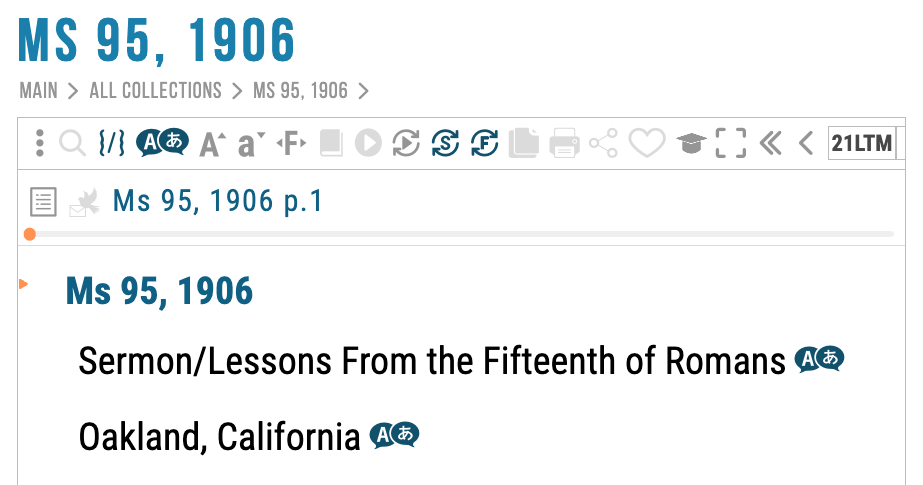
\includegraphics[width=1\linewidth]{images/sermons-and-talks.png}
    \label{fig:enter-label}
\end{figure}

Dla nas osobiście te cytaty są niepotwierdzone i nieważne, zwłaszcza w porównaniu z potwierdzonymi dziełami Ellen White. Lecz jeżeli ktoś nalega, aby traktować jej niepotwierdzone sprawozdania na równi z opublikowanymi pismami, nie będziemy się temu sprzeciwiać, ale jeszcze bardziej podkreślimy wniosek o Duchu Świętym jako istocie. Prześledźmy to razem.

Nawet w porównaniu z uwierzytelnionymi dziełami Ellen White, taki Duch Święty, istota, nie byłby jedno z Bogiem, ponieważ Chrystus był \egwinline{\textbf{jedyną istotą, która była jedno z Bogiem}}[Lt121-1897.7; 1897][https://egwwritings.org/?ref=en\_Lt121-1897.7&para=7266.13]. Ten Duch Święty, istota, nie mógłby \egwinline{\textbf{wejść we wszystkie rady i zamiary Boga}}, ponieważ Chrystus był \egwinline{\textbf{jedyną istotą}}[PP 34.1; 1890][https://egwwritings.org/?ref=en\_PP.34.1&para=84.75], która mogła to zrobić. Ta Istota nie ma być wywyższana, ponieważ \egwinline{\textbf{\underline{jedynie} Ojciec i Syn mają być wywyższeni}}[YI, 7 lipca 1898 akap. 2.; 1898][https://egwwritings.org/?ref=en\_YI.July.7.1898.par.2&para=469.2964]. Duch Święty, jako istota, nie pasowałby do porządku nieba jako trzecia istota, ponieważ Szatan był \egwinline{\textbf{zaraz po Chrystusie najbardziej wywyższoną \underline{istotą}} na niebiańskich dworach}[RH 9 sierpnia 1898, akap. 7; 1898][https://egwwritings.org/?ref=en\_RH.August.9.1898.par.7&para=821.17145]. Ten Duch Święty, istota, nie był zaangażowany w koszt zbawienia; nie był też w przymierzu z Ojcem i Synem, aby zbawić świat, ani nie został znieważony przez występek człowieka.

\egwinline{Wielki dar zbawienia został umieszczony w naszym zasięgu za \textbf{nieskończony koszt dla Ojca i Syna}.}[RH November 21, 1912, par. 2; 1912][https://egwwritings.org/?ref=en\_RH.November.21.1912.par.2&para=821.33329]

\egwinline{W planie ratowania zgubionego świata, rada była między nimi \textbf{\underline{oboma}}; \textbf{przymierze pokoju było między Ojcem a Synem}}[ST December 23, 1897, par. 2; 1897][https://egwwritings.org/?ref=en\_ST.December.23.1897.par.2&para=820.14803]

\egwinline{Ale w przestępstwie człowieka \textbf{\underline{zarówno} Ojciec, jak i Syn zostali znieważeni}.}[ST December 12, 1895, par. 7; 1895][https://egwwritings.org/?ref=en\_ST.December.12.1895.par.7&para=820.13243]

Taki Duch Święty, jako istota, nie jest zgodny z potwierdzonymi relacjami Ellen White ani z Pismem Świętym. Duch Święty jest nazywany ‘\textit{duchem}’, więc jest jedynie duchem.

Wiele cytatów siostry White pochodzi z kazań lub przemówień, które zostały opublikowane po jej śmierci. W dalszej części przedstawimy kilka, które są najczęściej omawiane w celu udowodnienia, że siostra White była trynitarianką. Zachęcamy wszystkich do porównania tych cytatów z jej potwierdzonymi i opublikowanymi za jej życia dziełami.

„\textit{A potem są dotykane złote harfy, a muzyka płynie przez wszystkie zastępy niebiańskie, i padają oni, oddając pokłon Ojcu i Synowi, i Duchowi Świętemu}.”\footnote{\href{https://egwwritings.org/?ref=en_Ms139-1906.32&para=9579.38}{EGW; Ms139-1906.32; 1906}} [Kazanie/Rozważania na temat Mt 4. Oakland, Kalifornia 24 lipca 1906; Wcześniej niepublikowane.]

„\textit{Musimy zdać sobie sprawę, że Duch Święty, który jest tak samo osobą, jak Bóg jest osobą, przechadza się po tych terenach.}”\footnote{\href{https://egwwritings.org/?ref=en_Ms66-1899.11&para=6622.19}{EGW; Ms66-1899.11: 1899}} [Przemówienie/Fragmenty przemówień wygłoszonych przez panią E. G. White podczas otwarcia College Hall, Avondale, oraz w kościele Avondale]
